\section{Conformal Probabilistic Safety Verification Method}\label{sec:conformal_method}
\vspace{-0.5em}
We now propose a \textit{conformal} probabilistic safety verification method for neural reachable tubes which is intended to be the direct analogue of the \textit{robust scenario-based} method in \sectionref{sec:scenario-based_method}.
The method is a straightforward application of split conformal prediction, a widely used method in the machine learning community for uncertainty quantification \citep{MAL-101}.

Using the same procedures as described in \sectionref{sec:scenario-based_method}, split conformal prediction can be used instead of robust scenario optimization to provide a probabilistic guarantee on the safety of the neural reachable tube and its complement, the neural safe set $\safeset$:
% In particular, the following theorem characterizes how the probabilistic safety guarantee is itself distributed according to the Beta distribution, which we prove in the Appendix of the extended version of this article:\textsuperscript{\ref{note:extended_paper}}
%In particular, the following theorem characterizes how the probabilistic safety guarantee is itself distributed according to the Beta distribution, which we prove in \appendixref{apd:conformal_theorem_proof}:
% 
\begin{theorem}[Conformal Probabilistic Safety Verification]
    \label{theorem:conformal_method}
    Let the number of outliers $k$ and the number of samples $N$ be as defined in the procedures in \sectionref{sec:scenario-based_method}, then:
\begin{equation}\label{eq:conformal_method_theorem}
        \underset{\state \in \safeset}{\mathbb{P}} \left( \costFunction(\state,0) > 0 \right) \sim \mathrm{Beta}(N-k, k+1)
    \end{equation}
\end{theorem}
% 
\theoremref{theorem:conformal_method} can be established via a straightforward application of conformal prediction with $-\costFunction(\state,0)$ as the scoring function. 
The proof is in the Appendix of the extended version of this article\textsuperscript{\ref{note:extended_paper}}. 
The above theorem states that the fraction of $\safeset$ that is safe is distributed according to the Beta distribution with shape parameters $N-k$ and $k+1$. 
Intuitively, the mass in the distribution shifts towards $0$ as $k$ increases for a fixed $N$, implying that it is more likely that a smaller fraction of $\safeset$ is safe, as expected.
For a fixed ratio $N:k$, $N$ controls how concentrated the mass is around the mean; i.e., for larger sample sizes $N$, we can more confidently determine the fraction of $\safeset$ that is safe.

% \begin{wrapfigure}{r}{0.3\columnwidth}
%   \centering
%   \vspace{-2em}
%   \includegraphics[width=0.3\columnwidth]{"figures/Figure 6"}
%   % \vspace{-2em}
%   \caption{The Beta distribution of $\underset{\state \in \safeset}{\mathbb{P}} \left( \costFunction(\state,0) > 0 \right)$ when $k=731$ outliers are found from $N=3684118$ samples. (Dashed black line) For an example choice of confidence $1-\beta=0.9$ (shaded blue), we can lower-bound the fraction of $\safeset$ which is safe with at least $1-\epsilon=0.99979$ ($99.979\%$) confidence.}
%   \vspace{-0.5em}
%   \label{fig:validation}
% \end{wrapfigure}
% 
To better understand \theoremref{theorem:conformal_method}, we show in \figureref{fig:beta} the Beta distribution of $\underset{\state \in \safeset}{\mathbb{P}} \left( \costFunction(\state,0) > 0 \right)$ for a solution learned by DeepReach on the multi-vehicle collision avoidance running example in \sectionref{sec:problem_setup}, for which $k=731$ outliers are found from $N=3684118$ samples.
% 
% %\vspace{-1.0em}
% \begin{SCfigure}[3.0][htbp]
%     \caption{The Beta distribution of $\underset{\state \in \safeset}{\mathbb{P}} \left( \costFunction(\state,0) > 0 \right)$ when $k=731$ outliers are found from $N=3684118$ samples. (Dashed black line) For an example choice of confidence $1-\beta=0.9$ (shaded blue), we can lower-bound the fraction of $\safeset$ which is safe with at least $1-\epsilon=0.99979$ ($99.979\%$) confidence.}
%     \includegraphics[width=0.25\columnwidth]{figures/Figure 6}
%     \label{fig:beta}
% \end{SCfigure}
% \vspace{-1.0em}
% % 
% 
% \vspace{-0.5em}
\begin{figure}[h!]
    \begin{minipage}[c]{0.23\textwidth}
       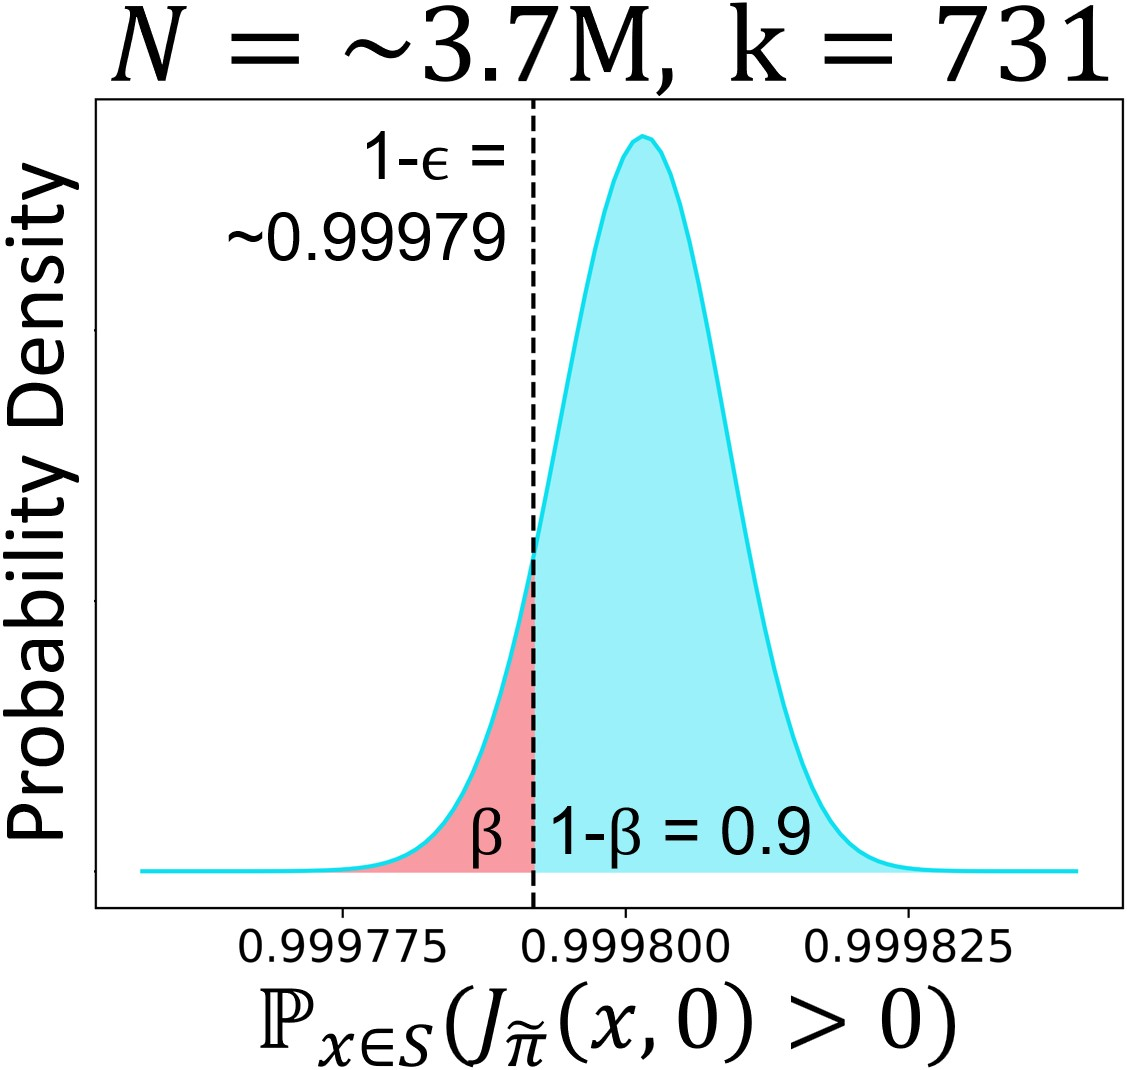
\includegraphics[width=\textwidth]{figures/Figure_6}
    \end{minipage}\hfill
    \begin{minipage}[c]{0.73\textwidth}
        \caption{The Beta distribution of $\underset{\state \in \safeset}{\mathbb{P}} \left( \costFunction(\state,0) > 0 \right)$ when $k=731$ outliers are found from $N=3684118$ samples. (Dashed black line) For an example choice of confidence $1-\beta=0.9$ (shaded blue), we can lower-bound the fraction of $\safeset$ which is safe with at least $1-\epsilon=0.99979$ ($99.979\%$) confidence.} \label{fig:beta}
    \end{minipage}
    \vspace{-1.0em}
\end{figure}
%


% 
\begin{remark} \label{remark:CP_coverage}
    The mean of the Beta distribution in Equation \eqref{eq:conformal_method_theorem} is given as $\frac{N-k}{N+1}$, which is roughly the fraction of the empirically safe samples. 
    One can immediately derive that the safety probability of $\safeset$, marginalized over the sampled ``calibration'' states, is given as: $\underset{ \left( \state_{1:N},\state \right) \in \safeset}{\mathbb{P}} \left( \costFunction(\state,0) > 0 \right) \ge \frac{N-k}{N+1}$, which precisely resembles the most commonly used \textbf{coverage property} of split conformal prediction.
\end{remark}
% 

Even though \theoremref{theorem:conformal_method} provides the distribution of the safety level, when we compute safety assurances in practice, it is often desirable to know a lower-bound on the safety level with at least some desired confidence.
This corresponds to choosing a lower-bound whose accumulated probability mass is smaller than some confidence parameter $\beta$ (shaded red in \figureref{fig:beta}).
The following lemma formalizes this by using the CDF of the Beta distribution in \theoremref{theorem:conformal_method}. 
% and which we prove in the Appendix of the extended version of this article:\textsuperscript{\ref{note:extended_paper}}
%This leads us to introduce the following lemma, which we prove in \appendixref{apd:conformal_lemma_proof}:
\begin{lemma}[Conformal Probabilistic Safety Verification]
    \label{lemma:conformal_method}
    Select a safety violation parameter $\epsilon \in (0, 1)$ and a confidence parameter $\beta \in (0, 1)$ such that
    \begin{equation} \label{eq:conformal_method_lemma}
        \begin{aligned}
            \sum^k_{i=0} \binom{N}{i} \epsilon^i (1-\epsilon)^{N-i} \le \beta
        \end{aligned}
    \end{equation}
    where $k$ and $N$ are as defined above. 
    Then, with probability at least $1-\beta$, the following holds:
    \begin{equation} \label{eq:conformal_method_lemma_guarantee}
        \begin{aligned}
            \underset{\state \in \safeset}{\mathbb{P}} \left( \vfunc(\state,0) \le 0 \right) \le \epsilon
        \end{aligned}
    \end{equation}
\end{lemma}
\lemmaref{lemma:conformal_method} is, in fact, precisely the same result as obtained by \theoremref{theorem:scenario-based_method} using robust scenario optimization.
This is no coincidence, as one can show that split conform prediction more generally reduces to a robust scenario-optimization problem.
% 
\begin{remark}
    In general, a split conformal prediction problem can be reduced to a robust scenario-optimization problem. This is proven in the Appendix of the extended version of this article.\textsuperscript{\ref{note:extended_paper}}
\end{remark}
% 
Due to the equivalence between conformal method and robust scenario-based methods, the analysis in \sectionref{sec:scenario-based_method} holds here as well.
More generally, we hope that this insight will lead to future research into further investigating the close relationship between the two methods.